\chapter{Elméleti háttér és irodalomkutatás}

Ebben a fejezetben kerül bemutatásra minden jelentősebb alapfogalom, valamint az azokhoz szorosan kapcsolódó technikák és folyamatok, amelyek ismerete nélkülözhetetlen a videó streaming megértéséhez, illetve annak szoftveres megvalósításához.

\section{A videó formátumai}

A videó egy multimédiás eszköz auditív és mozgó vizuális információ tárolására, visszajátszására. Fontos felhasználási területei a bevezetésben is ismertetett média- és a szórakoztató ipar.

Egy videó tartalmazhat különböző nyelvű hanganyagokat, mozgóképet, és egyéb metaadatokat -- például feliratokat és miniatűr állóképeket -- mind egy fájlban. Ezek közös tárolására konténerformátumokat alkalmazunk, amelyek megadják, az egyes adatfolyamok hogyan, milyen paraméterekkel, kódolással, tömörítéssel kerüljenek tárolásra, és hogyan kerülhetnek majd lejátszásra.

Szokásos összekeverni, de a konténerformátumoktól függetlenül a mozgóképkódolás és a hangkódolás különálló folyamatok. A kódolás egy algoritmus nyomán az adatot tömöríti, hogy a tárolás és a továbbítás hatékonyabb legyen.

\subsection{Konténerformátumok}

A legelterjedtebb és legszélesebb körben támogatott konténerformátum a Moving Picture Experts Group (MPEG) gondozásában specifikált MP4 -- avagy a sztenderdben használt nevén: MPEG-4 Part 14 --, amely az MPEG-4 projekt részeként született 2001-ben.

Ugyancsak az MPEG gondozásában, az MPEG-2 projekt részeként született 1995-ben az MPEG Transport Stream (MPEG-TS) konténerformátum, amely elsősorban a digitális televíziózásban használatos, és így az internetes videó streaming során is. Felbontja a videóadatokat kisebb, fix hosszú adatcsomagokra, ezzel is előkészítve a tulajdonképpeni kis késleltetésű azonnali továbbítására a videóanyagnak a hálózaton keresztül.

További elterjedt konténerformátumok közé tartozik a Matroska Video (MKV), amely a hibatűréséről ismert; Apple vállalat által macOS-re és iOS-re optimalizálva fejlesztett QuickTime Movie (MOV) formátuma; valamint a WebM, egy szabad felhasználású webes kiszolgálásra optimalizálódott formátum, amelyet nagyobb jelentőségű webböngészők mind támogatnak. Régebbi, már kevésbé használt vagy kivezetett formátumok közé tartozik az Audio Video Interleave (AVI) és a Flash Video (FLV).

\subsection{Mozgókép kódolási módszerei}

Az MPEG-4 projekt keretében született az Advanced Video Coding (AVC) -- avagy H.264 -- kódolási szabvány mozgókép kódolására, amely 2004-ban vált elérhetővé. Továbbra is ez az egyik legelterjedtebb szabvány, a videó streamingben használt konténerformátumok is ezt a kódolást alkalmazzák.

Természetesen azóta több új szabvány is megjelent hasonlóan az MPEG projektjei alatt, mint például az 2013-ban megjelent High Efficiency Video Coding (HEVC) -- avagy H.265 --, amely az AVC-től jobb tömörítést és jobb minőséget ígér, de a licencdíjak miatt nem vált annyira elterjedtté, mint az elődje.

Ezen modern problémák kiküszöbölésére terjedt el a VP8 és a VP9 -- a WebM formátumnak tagjaként --, illetve az AV1 szabad felhasználású kódolási szabványok.

A szabványok konkrét megvalósításával (kodekek) nem foglalkozunk részletesebben, de egy szabad felhasználású és nyílt forráskódú megvalósítása a H.264-nek a x264, amelyet például az FFMpeg szoftvercsomag is használ videó kódolására és dekódolására.

\subsection{Hang kódolási módszerei}

Hanganyag kódolására is több szabványt tudunk megvizsgálni. Ilyen az MPEG Audio Layer III -- rövid nevén: MP3 -- 1991-ből, ezt 1997-ben az Advanced Audio Coding (AAC) szabvány váltotta le. Ezen szabványok az MPEG által kerültek kifejlesztésre, valamint mindkettő veszteséges tömörítést alkalmaz, azaz a kódoláson és dekódoláson átesett hanganyag minősége nem lesz azonos az eredeti hanganyaggal.

Főleg a mozivilágban használt kódolás a Dolby AC-3 -- ismertebb nevén: Dolby Digital. Azonos bitrátánál is az előbbieknél jobb minőséget ígér. 2017-ben már lejárt a szabadalmi védelme, így azóta szabadon felhasználható. Egy másik, születése (2012) óta szabad felhasználású kódolás az Opus, amelyet a Skype és a Discord is használ VoIP-alapú kommunikációra, és az összes eddig említett kódolásnál jobb minőséget produkál.

Természetesen találkozhattunk tömörítetlen (pl.: WAV), illetve veszteségmentes kódolásokkal is (pl.: FLAC) is, azonban a streaming világában ezek nem használatosak, mivel a nagyobb fájlméretük meghaladná a sávszélesség és a tárhely korlátait. Az AC-3 és AAC szabványok közül szokás választani a videó streaming során, széles körben kompatibilisek mindenféle lejátszó eszközzel, míg az Opus még nem eléggé támogatott.

\section{Videó streaming kiszolgálása}\label{streamref}

A média streaming egy olyan folyamat, amely során az médiaadatokat -- mi esetünkben videóadatot -- egy adott hálózati protokoll felett, egy adott konténerformátumban, adott kódolásssal továbbítjuk a végfelhasználók számára. Elsősorban az azonnali elérhetőségre összpontosít, azaz a lejátszásnak a lehető legkisebb késleltetéssel kell megtörténnie, kevésbé fontos a streaming során a minőség megtartása, mint ahogy az fontos lenne teljes médiumok egyben való letöltésekor.

A streaming során az adatfolyamba helyezés előtt a videóadatokat újrakódoljuk, majd kisebb adatcsomagokra -- úgynevezett ``packetekre'' -- bontjuk, és ezeket a csomagokat a hálózaton keresztül továbbítjuk a végfelhasználók felé. Az adatcsomagok önmagukban is értelmezhetőek, és a végfelhasználók lejátszó alkalmazásai képesek az adatcsomagokat a megfelelő sorrendben és időzítéssel lejátszani. A streaming könnyen reagál a lejátszás során ugrálásokra, előre- és visszatekerésre, mivel a videót nem kell teljes egészében letölteni a végfelhasználói eszközre, hanem a feldarabolt videócsomagot a lejátszás során továbbítjuk abban a pillanatban, amikor arra szükség lesz.

\subsection{Az élő közvetítés és Video-on-Demand különbségei}

Annak megfelelően, hogy az adat egésze mikor áll rendelkezésünkre, kettő fő streaming típust különböztetünk meg: az élő közvetítést (live streaming) és a Video-on-Demand (VOD) streaminget. A VOD esetében a videóadatokat előre rögzített formában tároljuk, és a végfelhasználók a videóadatokat a saját időbeosztásuknak megfelelően nézhetik meg. Az élő közvetítés esetében a videóadatokat valós időben továbbítjuk a végfelhasználók felé, és a végfelhasználók a videóadatokat a közvetítés során nézhetik meg.

Különbözik mindkettőnél, hogy milyen fizikai infrastrukturális tervezést kell végrehajtani a legjobb kiszolgálás érdekében. Élő adásoknál a késleltetés a középponti kihívás, mivel a videóadatokat a lehető leggyorsabban kell továbbítani a végfelhasználók felé, hogy a közvetítés valóban élőnek tűnjön, ehhez magas számítási teljesítmény szükséges. A VOD esetében a hálózati sávszélességből adódó problémák leküzdése a központi kihívás, mivel a videót a felhasználók sokkal nagyobb közönsége kívánja elérni, azt kiváló minőségben szeretné megtekinteni, ennek ellenére a globális sávszélesség korlátozott. Itt a caching és a tartalomterjesztés optimalizálása a kulcs, ekkor jönnek képbe a Content Delivery Networkök (CDN-ek), azaz a tartalomterjesztő hálózatok. \cite{cdn}

Üzleti szempontból a bevétel az élő adások során a közbeiktatott reklámokból származik főleg és a pay-per-view rendszerekből, míg a VOD esetében a közbeiktatott reklámokon kívül a felhasználók előfizetési díjából, tranzakcionális egyszeri vásárlásból -- amennyiben a reklámokat kerülni szeretnék.

Lentebb két ábrát (\refstruc{fig:vodsetup} és \refstruc{fig:livesetup}) láthatunk, amelyek absztrakt példákat mutatnak egy VOD-kiszolgálás és egy élő közvetítés résztvevő médiaeszközeire. A rajta feltüntetett protokollok és fájlnevek a későbbi alfejezetekben olvasása során érthetőek lesznek.

\begin{figure}[h]
	\centering
	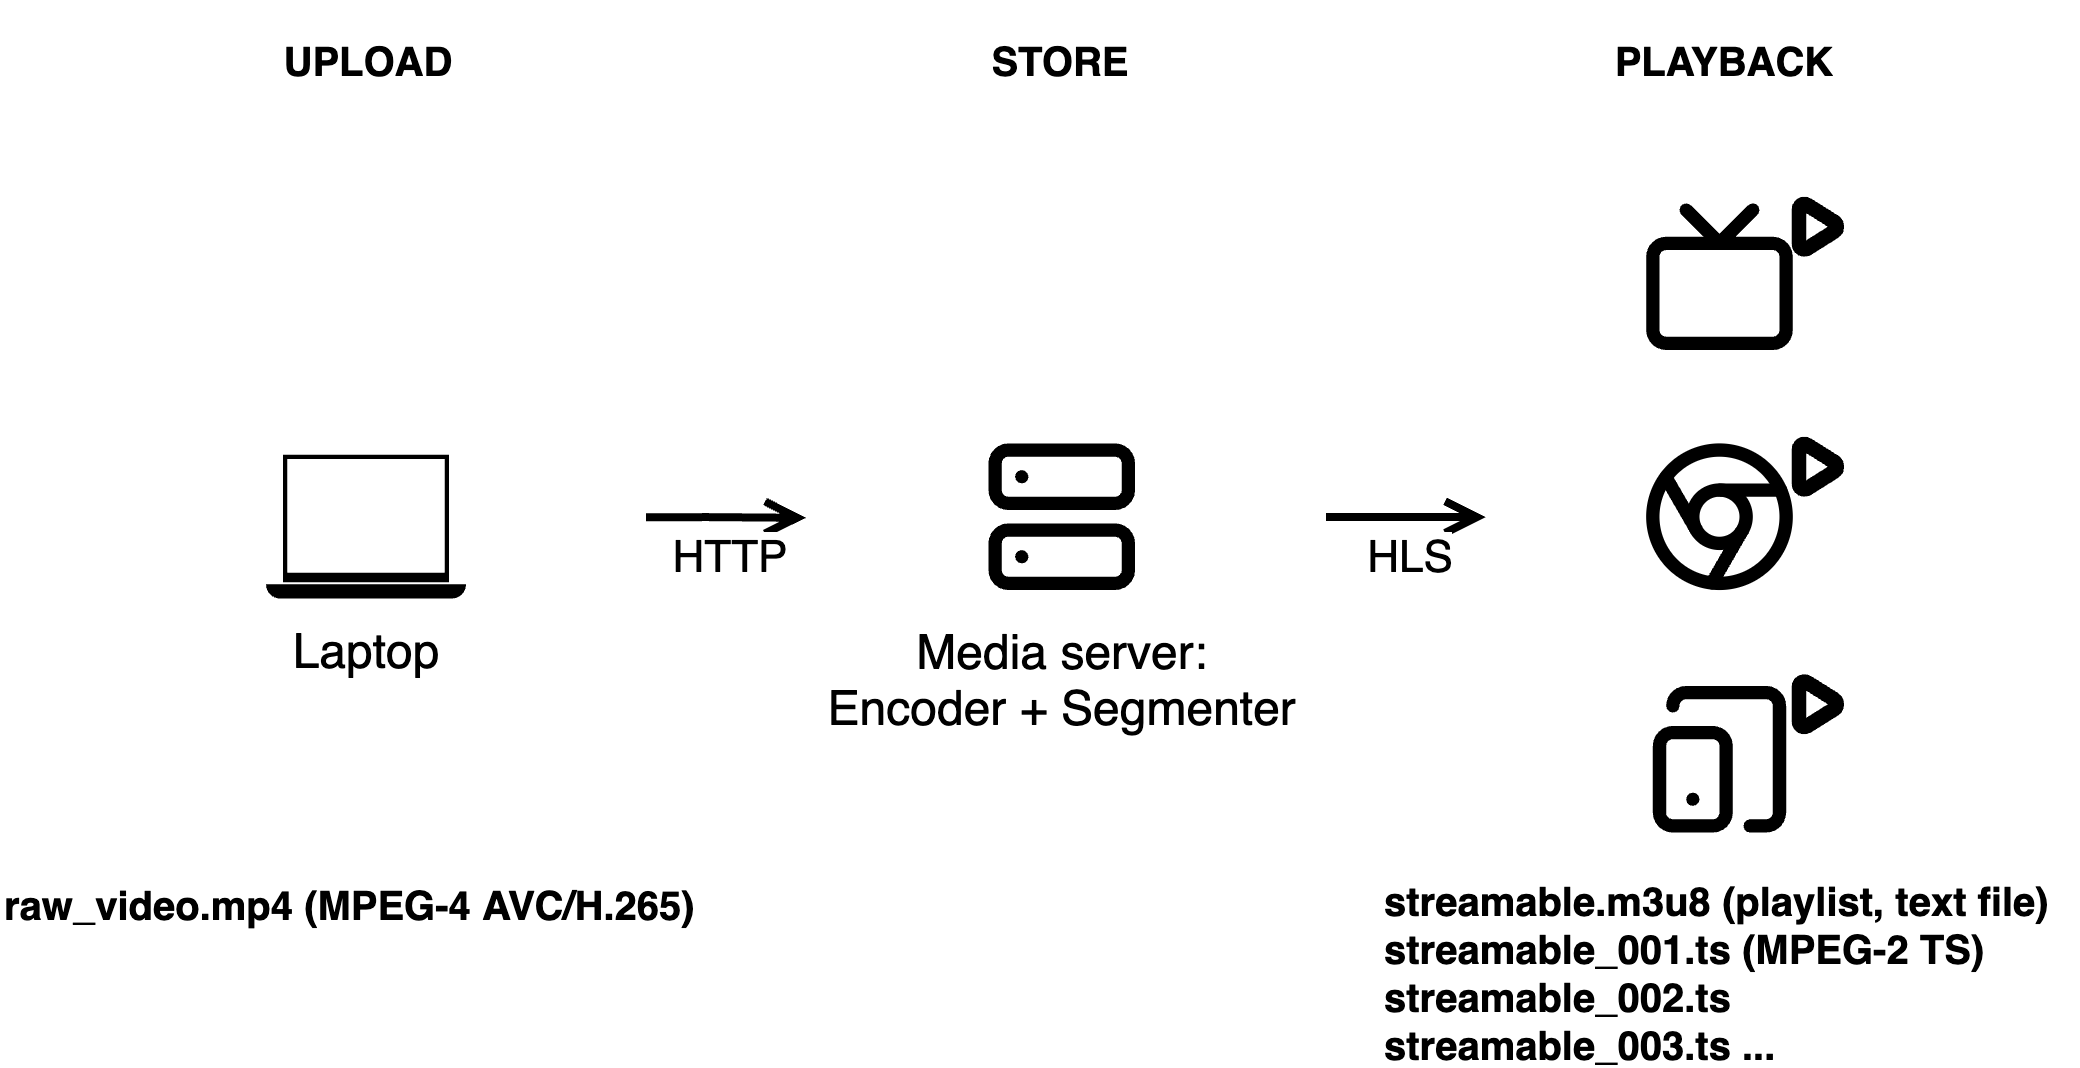
\includegraphics[width=120mm, keepaspectratio]{figures/dipterv_vodsetup.png}
	\caption{Példa egy VOD-kiszolgálás résztvevő eszközeire.}
	\label{fig:vodsetup}
\end{figure}

\begin{figure}
	\centering
	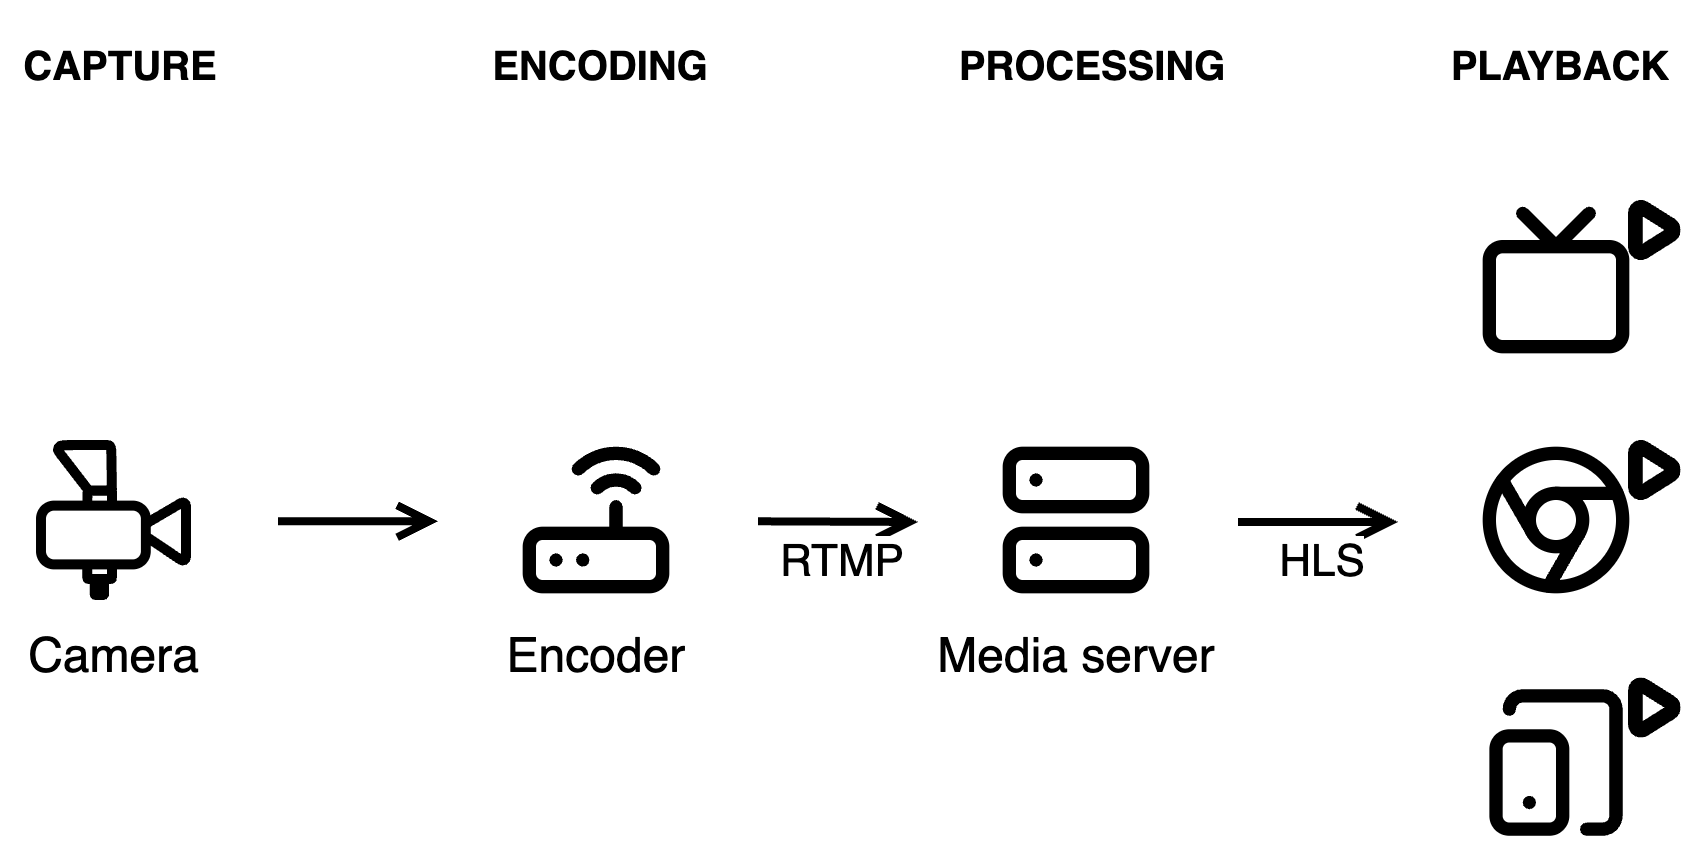
\includegraphics[width=100mm, keepaspectratio]{figures/dipterv_livesetup.png}
	\caption{Példa egy élő közvetítés résztvevő eszközeire.}
	\label{fig:livesetup}
\end{figure}

\subsection{Adaptive Bitrate Streaming}

A streamelést erősen befolyásoló tényező a hálózati feltételek változása, amelyek a videólejátszás minőségét és késleltetését is befolyásolják. Az Adaptive Bitrate Streaming (ABR) egy a hálózati kiszolgálás során alkalmazott technika, amely megoldást jelenthet erre a problémára.

Az ABR során a forrásvideót több különböző bitrátával dolgozó kodekekkel és különböző felbontással kódoljuk a médiaszerveren, majd lejátszáskor a lejátszó alkalmazás a hálózati feltételek változására reagálva, valamint a fogadó fél számítási kapacitásától függően valós időben választja ki a megfelelő vi\-de\-ó\-strea\-met ezek közül, onnan válogatja a packeteket (\refstruc{fig:ABR}).

\begin{figure}
	\centering
	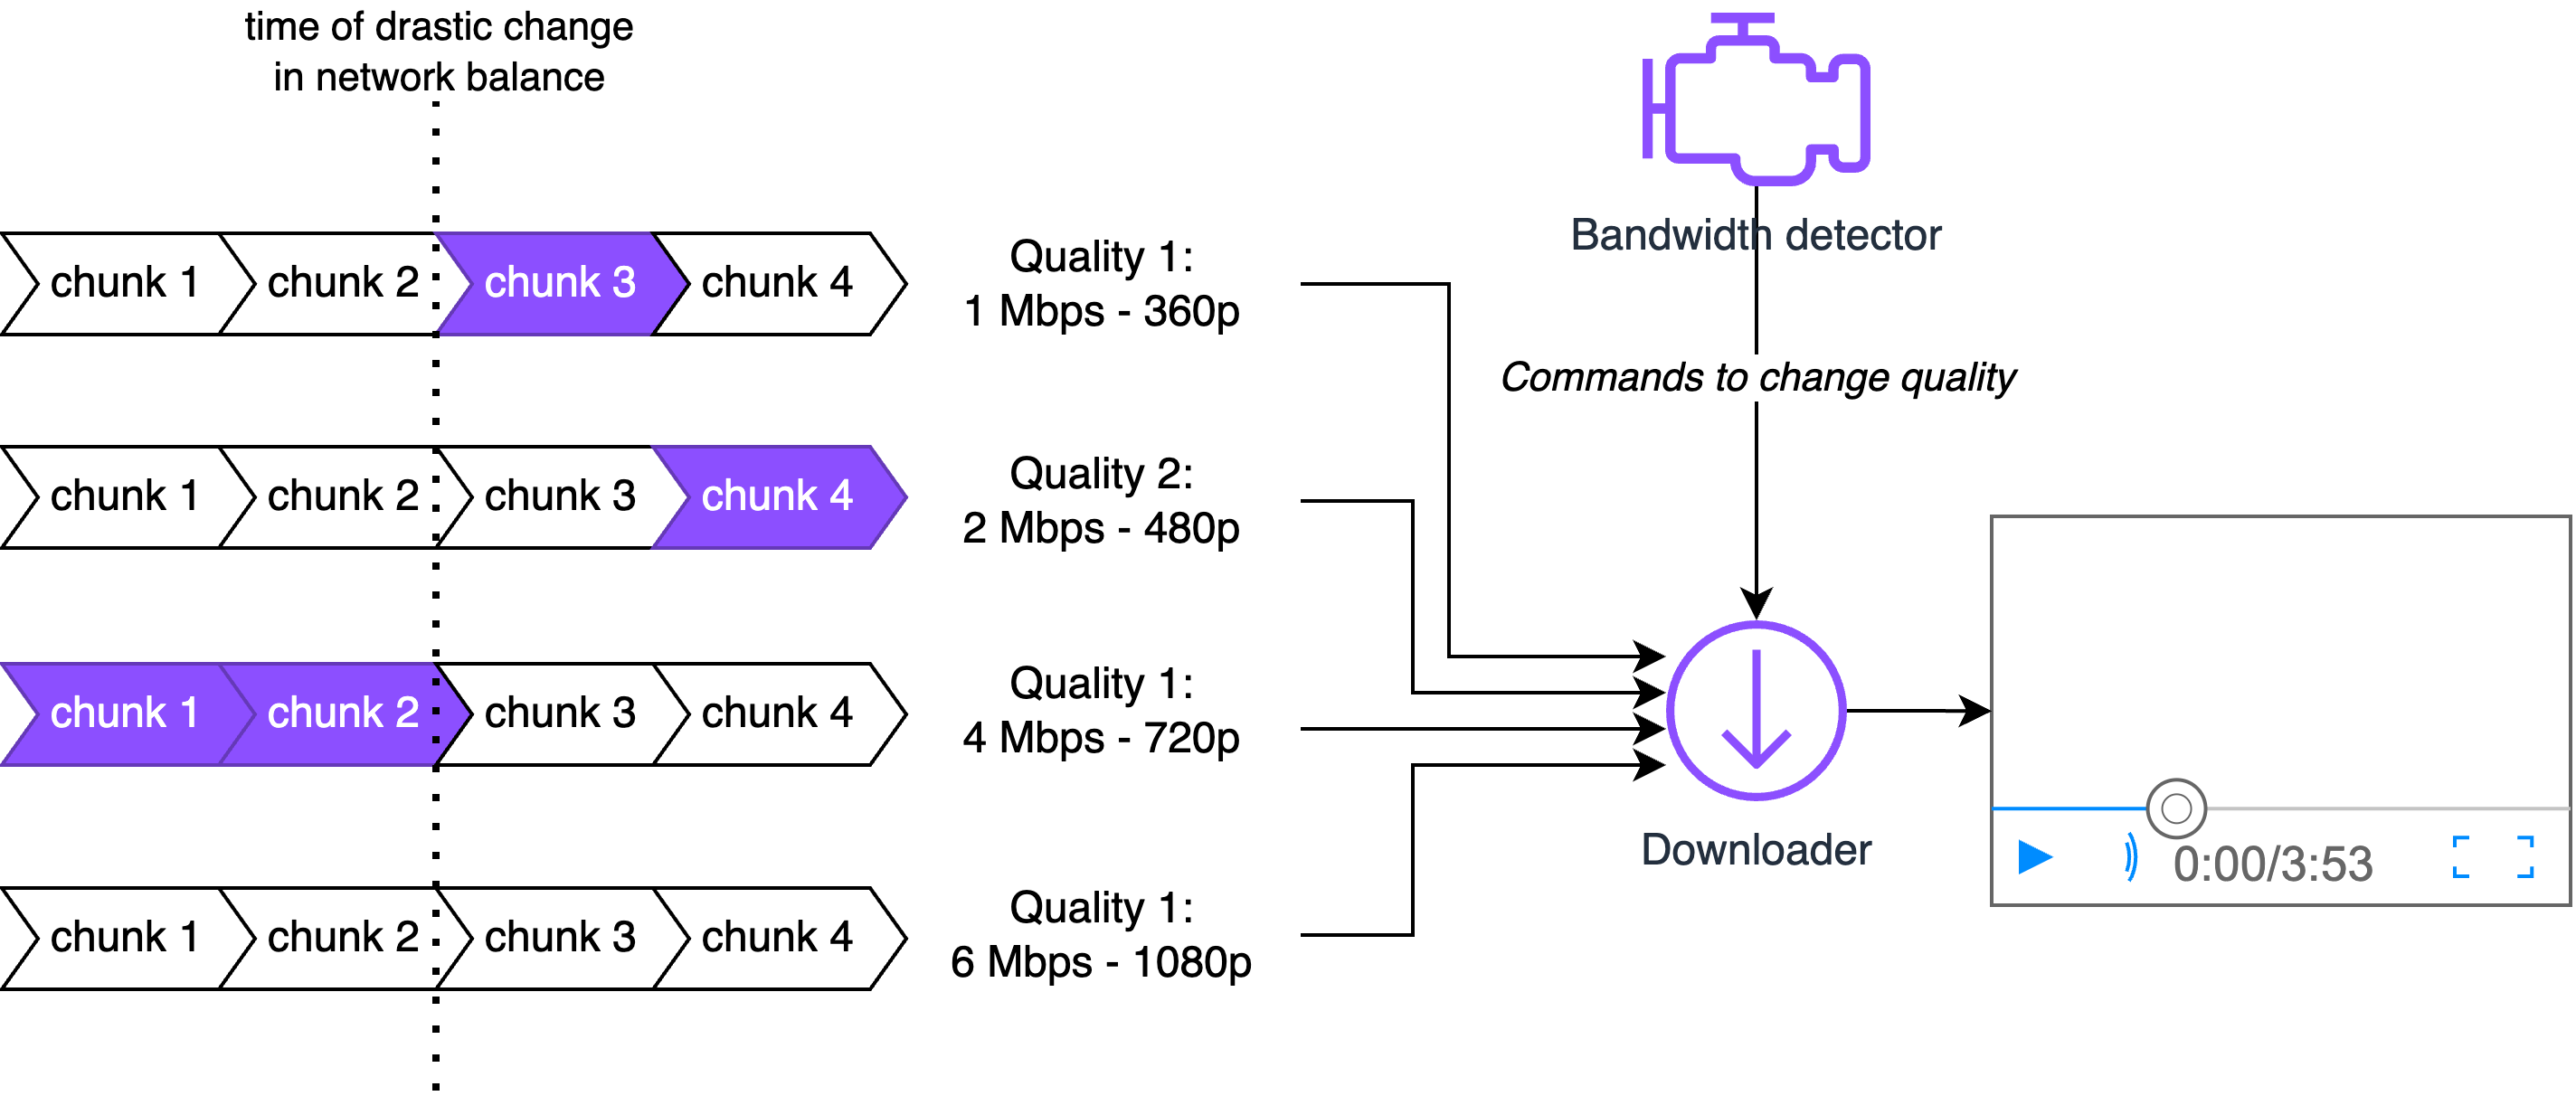
\includegraphics[width=140mm, keepaspectratio]{figures/dipterv_abr.png}
	\caption{Az Adaptive Bitrate Streaming működése.}
	\label{fig:ABR}
\end{figure}

Tiszta, hogy az ABR-t megvalósító rendszer előnyös mind a VOD, mind az élő közvetítés esetében, mivel a hálózati feltételek változása mindkét esetben előfordulhat, az automatikus streamváltogatás beavatkozás nélkül sokkal nagyobb Quality of Experience (röviden QoE, magyarul \emph{az élmény minősége}) lehetőségét tudja biztosítani \cite{DashAbr}. Az ABR-t alkalmazó rendszerek a videóadatokat több különböző bitrátával kódolják, ez természetesen a feldolgozási idejét a rendszereknek megnöveli, sőt élő közvetítés során egységnyi idő alatt jóval több számítási terhelést kell kibírnia a rendszernek.

\section{Videó streaming hálózati protokolljai}

Videó streamelésére -- másképp fogalmazva: valamely korábban ismertetett formátumban tárolt videófájl adatfolyamba való illesztésére -- különböző hálózati protokollok palettája áll rendelkezésünkre.

Néhány ismertebb célprotokoll létrejöttük időrendjében \cite{StreamingHistory}:

\begin{itemize}
	\setlength{\itemsep}{1pt}
  \setlength{\parskip}{0pt}
  \setlength{\parsep}{0pt}
	\item Real-Time Messaging Protocol (RTMP, 1996)
	\item Microsoft Smooth Streaming (MSS, 2008)
	\item Adobe's HTTP Dynamic Streaming (HDS, 2009)
	\item HTTP Live Streaming (HLS, 2009)
	\item WebRTC (2011)
	\item Dynamic Adaptive Streaming over HTTP (DASH, 2012)
\end{itemize}

Jelen alfejezet ezen alkalmazásrétegben alkalmazott protokollok (Layer 7) közül vizsgálja meg a legelterjedtebbeket, kitérve arra is, milyen szállítási rétegű protokollokkal (Layer 4) tudnak együttműködni.

\subsection{Real-Time Messaging Protocol}

A Real-Time Messaging Protocolt (RTMP) nevű protokollt még a Macromedia nevű cég fejlesztette ki, amely vállalatot később az Adobe felvásárolta. Az RTMP egy teljes szervertől kliensig tartó protokoll, amely a Flash Player és a Flash Media Server közötti kommunikációra lett kifejlesztve eredendően. Közvetlen dolgozik a TCP felett, ennek nincs köze a HTTP-hez. \cite{StreamingHistory} Az RTMP-t még támogatja sok-sok platform, mert egész alacsony késleltetést lehet vele elérni, egészen alacsony ``költségű'', a Twitch és a YouTube is támogatja, hogy RTMP pull üzemmódjában tudjunk ezeken a platformokon élő adást fogadni, tehát szerveroldalon még használt, persze a Flash Player támogatásának 2020-as kivezetése miatt a protokoll használata kliensoldalon pedig visszaszorult.

\subsection{HTTP Live Streaming}

A HTTP-alapú streaming protokollok közül a legelterjedtebb a HTTP Live Streaming (HLS), amelyet az Apple fejlesztett ki 2009-ben. A HLS eredetileg az Apple jogvédett kereskedelmi protokolljaként indult, azóta viszont már szabad felhasználásúvá vált. Az Apple eszközök -- macOS, iOS -- alapértelmezetten támogatják ezt a protokollt, és a modern böngészők is támogatják a Media Source Extensions (MSE) API-n keresztül. Az HLS a HTTP felett dolgozik, egymástól függelten packetekre szedi a teljes kiszolgálandó videót, és az RTMP-hez képest ez így állapotmentes adatforgalmazást tud megvalósítani. \cite{StreamingHistory}

HLS használata során H.264 formátumban kell a videóadatokat kódolni, a hangot AAC, MP3 vagy Dolby szabványokkal lehet kódolni. A konténerformátumot tekintve is kötött, MPEG-2 Transport Stream (MPEG-TS) formátumot használhatjuk, vagy pedig az MP4-et -- fMP4 technikával, azaz \emph{fragmented MP4-gyel}, ehhez pedig a Common Media Application Format (CMAF) konténerformátumra kell átalakítani. \cite{Cmaf} A darabokra szedést követően a packeteket egy lejátszási listában (.m3u8 kiterjesztésű szöveges indexfájl) tartja számon a szerver, amelyet a lejátszó alkalmazások letöltenek, és a lejátszás során a megfelelő sorrendben és időzítéssel lejátszák. \cite{HlsApple} Lásd a példát egy 720p-s streamet leíró indexfájlra a \ref{lst:m3u8example}. kódrészletben.

A HLS egy olyan protokoll, amely magában hordozza az ABR implementációját is, kliensoldalon modern Media Source Extensions funkcionalitást támogató böngészőkben elterjedt használni a \emph{hls.js}\footnote{\url{https://github.com/video-dev/hls.js}} nevű JavaScript-könyvtárat, amely implementálja a HLS protokollt. A .m3u8 indexfájl definiálhat több másik ilyen indexfájlt is, amelyek a különböző bitrátájú videóstreameket képviselik (pl. egy \emph{1080p.m3u8} fájl és egy \emph{720p.m3u8} fájl írja le a playlistjét egy-egy bitrátájú streamnek).

\vspace{0.4cm}
\begin{lstlisting}[caption=Részlet egy .m3u8 indexfájlból.,label=lst:m3u8example,basicstyle=\small,]
#EXTM3U
#EXT-X-VERSION:3
#EXT-X-TARGETDURATION:4
#EXT-X-MEDIA-SEQUENCE:1
#EXTINF:4.000000,
skate_phantom_flex_4k_2112_720p1.ts
#EXTINF:4.000000,
skate_phantom_flex_4k_2112_720p2.ts
#EXTINF:4.000000,
skate_phantom_flex_4k_2112_720p3.ts
#EXTINF:4.000000,
skate_phantom_flex_4k_2112_720p4.ts
#EXTINF:4.000000,
skate_phantom_flex_4k_2112_720p5.ts
\end{lstlisting}

\subsection{Dynamic Adaptive Streaming over HTTP}

A Dynamic Adaptive Streaming over HTTP -- DASH vagy MPEG-DASH, tekintve a fejlesztője ennek is az MPEG csoport volt -- egy 2012-ben szabványosított protokoll. Hasonlít a HLS-hez, HTTP felett forgalmaz, sorozatba illeszt egymástól független packeteket. Ezeket a szegmentált packeteket egy manifestfájlban tartja számon a szerver (Media Presentation Description, MPD-fájl). \cite{Dash}

A HLS-hez képest ez a protokoll kodekagnosztikus, ami annyit jelent, hogy nem kötődik videókodekhez, használható H.264, H.265, akár VP9 is. \cite{DashIso} Igyekeztek ezzel a protokollal egyezményesíteni a tartalomvédelmet is, Common Encryptiont (CENC) használ titkosításra. Digitális jogkezelésre (Digital Rights Management, DRM) is agnosztikus. Amióta a HLS támogatja az CMAF konténerformátumban való szállítást, azóta könnyen át lehet arról állni akár DASH protokollra is, ugyanis a DASH is CMAF-alapú. A DASH a HTTP/2 protokollt is támogatja, sőt HTTP/3-at is már UDP felett.

A HLS-hez hasonló elvekkel dolgozik a DASH is, illetve ez is egy ABR technológiájú protokoll. A DASH implementációjára JavaScript motorral rendelkező kliensekben -- böngészők, mobiltelefonok stb. -- a \emph{dash.js}\footnote{\url{https://dashjs.org/}} könyvtárat használják legtöbb esetben.

\subsection{WebRTC}

A WebRTC (Web Real Time Communications) egy nyílt forráskódú projekt részeként alapult -- támogatják kódbázisának fenntartását mind a Google, a Mozilla és az Opera csapatai is --, egy protokoll böngészőalapú valós idejű kommunikáció kialakítására. Ezt használja a Discord, a Google Chat és egyéb webes videóchat-alkalmazások. \cite{StreamingHistory}

A források és a streamet figyelők számának kardinalitása szempontjából ez eltér az előzőekben ismertetettektől -- amelyek egy forrás és több befogadóra optimalizált --, ez viszont peer-to-peer (P2P) alapú, tehát oda-vissza jellegű streamlést kell biztosítson, emiatt a WebRTC a legjobb választás, amennyiben a felhasználási célja az, hogy a felhasználók közvetlenül egymással kommunikálhassanak, és nem szükséges közbeiktatni egy központi médiaszervert. Ezenkívül a WebRTC-t egyre szélesebb körben próbálják alkalmazni a videó streaming területén is one-to-many közvetítésre is. Szabad felhasználású kodekeket alkalmaz videó- és hangkódolás terén (pl.: Opus, VP9). \cite{WebRTC}
